\documentclass[a4paper,11pt,fleqn]{article}%fleqn pour aligner les equations à gauche
\usepackage{../../Styles/Cours}


\newcommand{\chnum}{Chapitre 16}
\newcommand{\chtitle}{Thermodynamique}
\newcommand{\dtype}{Cours}
  

\begin{document}
	\maketitle
	\section{Modèle du gaz parfait}
	\subsection{Définitions du modèle}
	La différence la plus frappante entre les différents états de la matière est la masse volumique $\rho$ : pour un gaz, elle est d'environ \SI{1}{\kilo\gram\per\meter\cubed}. Cela est stypiquement 1000 fois plus faible que la masse volumique d'un solide ou d'un liquide (de $10^3$ \unit{\kilo\gram\per\meter\cubed} à $10^4$ \unit{\kilo\gram\per\meter\cubed}). La masse volumique $\rho$ renseigne sur la distance qui sépare les particules à l'échelle microscopique.\\
	En thermodynamique, on définit la température $T$, exprimée en kelvin (\unit{K}), comme proportionnelle à l'énergie cinétique microscopique moyenne des molécules.\\
	La pression $p$, en pascal (\unit{\pascal}), permet de mesurer l'intensité des chocs des molécules de gaz avec la paroi du récipient qui les contient. Elle est d'autant plus faible que le gaz est dilaté.
	\subsection{Équation d'état d'un gaz parfait}
	Pour étudier un système gazeux, on peut se placer dans le cadre du modèle du gaz parfait : on assimile les molécules du gaz à des points matériels et qui suppose qu'il n'y a aucune interaction entre les molécules. Ce modèle permet d'établir une équation reliant différentes variables d'état, appelée équation d'état du gaz parfait :
	\begin{center}
		\begin{tabular}{c|l}
	\multirow{5}{*}{$p \cdot V = n \cdot R \cdot T$} & $p$ : pression du gaz parfait (\unit{\pascal})\\
	& $V$ : volume du gaz parfait (\unit{\meter\cubed})\\
	& $n$ : quantité de matière de gaz parfait (\unit{\mole})\\
	& $R$ : constante des gaz parfaits égale à $R = \SI{8,314}{\joule\per\mole\per\kelvin}$\\
	& $T$ : température du gaz parfait (\unit{\kelvin})\\
		\end{tabular}
	\end{center}
	\subsection{Limites du modèle}
	Comme tout modèle, le gaz parfait ne permet pas de décrire avec justesse un gaz, quelles que soient les conditions. À haute pression, on ne peut plus négliger le volume occupé apr les molécules devant le volume occupé par le gaz. Par ailleurs, pour certains gaz, il existe des interactions importantes entre les molécules du gaz. Enfin, à basse température, l'énergie cinétique devient trop faible : on ne peut plus négliger l'énergie d'interaction. D'autres modèles permettent alors une description plus adaptée.
 
	\section{Énergie interne}
	\subsection{Définition}
	A l'échelle \underline{macroscopique}, un système possède une énergie mécanique qui résulte de son énergie cinétique et de don énergie potentielle.\\
	A l'échelle \underline{microscopique}, chacune entité constituant le système possède :
	\begin{itemize*}
		\item une énergie cinétique liée à l'agitation
		\item une énergie potentielle liée aux interactions en son sein et aux interactions avec les autres entités.
	\end{itemize*}
	Le système possède alors une \textbf{énergie interne}, notée $\mathbf{U}$, somme des énergies cinétiques et potentielles de toutes les entités microscopiques qui le constituent. On peut écrire :
	$$U = E_c(micro) + E_p(micro)$$
	Remarque : l'énergie interne n'est pas calculable directement car il serait très complexe d'appréhender le comportement de toutes les entités constituant un système. Néanmoins, il est possible de déterminer sa variation.\\
	L'\textbf{énergie totale} d'un système est la somme de son énergie mécanique d'origine macroscopique et de son énergie interne d'origine microscopique. On a :
	$$E_{tot} = Em + U$$
	
	\subsection{Transferts d'énergie}
	Un système peut échanger de l'énergie avec son environnement extérieur.
	
	\noindent \begin{minipage}{.8\linewidth}
		\begin{itemize}
			\item La quantité d'énergie échangée au niveau macroscopique se mesure grâce au \textbf{travail} $\mathbf{W}$.\\ \textcolor{gray!70}{Exemple : lorsqu'il est comprimé, le gaz contenu dans une seringue reçoit une énergie égale au travail de la force pressante ayant servi à le comprimer.}
			\item La quantité d'énergie échangée au niveau microscopique correspond à un \textbf{transfert thermique}. Celui-ci s'effectue spontanément du système le plus chaud vers le système le plus froid. La \textbf{quantité d'énergie thermique} ainsi \textbf{transférée} est notée \textbf{Q}.\\
			La vitesse de transfert thermique est évaluée grâce au \textbf{flux thermique} $\mathbf{\phi}$ :\\
			
			\begin{tabular}{c|m{10cm}}
				\multirow{3}{3cm}{$\mathbf{\phi = \dfrac{Q}{\Delta t}}$} & $\phi$ : flux thermique (en W)\\
				&$Q$ : énergie thermique transférée (en J)\\
				&$\Delta t$ durée (en s)\\
			\end{tabular}\\
			
			Remarque : le flux thermique est homogène à une puissance. on peut donc aussi parler de puissance thermique.
		\end{itemize}
	\end{minipage}
	\begin{minipage}{.2\linewidth}
		\centering
%		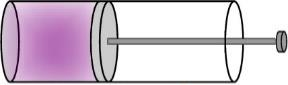
\includegraphics[scale=.35]{Ressources/TSPE_C14_Cours_Fig1.png}\\
		\vspace{4cm}
%		
\includegraphics[scale=.35]{Ressources/TSPE_C14_Cours_Fig2.png}
	\end{minipage}

	Par convention, le travail, le transfert thermique $Q$ et le flux thermique $\phi$ sont comptés :
	\begin{itemize*}
		\item positivement s'ils sont reçus par le système
		\item négativement s'ils sont cédés par le système
	\end{itemize*}
\begin{center}
	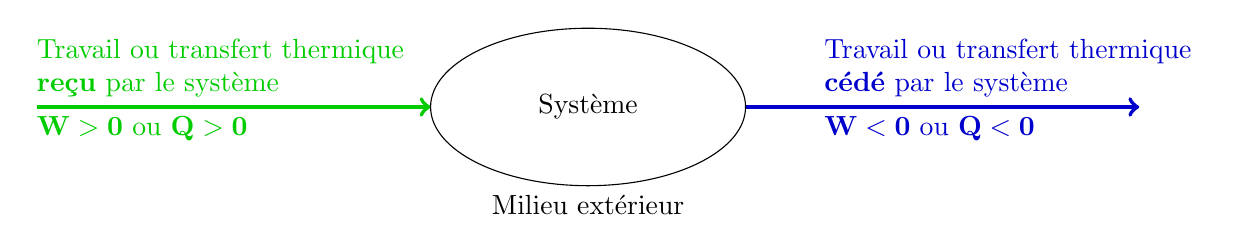
\begin{tikzpicture}
		\draw[green!80!black,->,line width=1.5] (-7,0) to (-2,0);
		\draw[blue!80!black,->,line width=1.5] (2,0) to (7,0);
		\draw (0,0) ellipse (2 and 1);
		
		\draw[green!80!black] (-4.5,0) node[above,text width=5cm]{Travail ou transfert thermique \textbf{reçu} par le système};
		\draw[green!80!black] (-4.5,0) node[below,text width=5cm]{$\mathbf{W>0}$ ou $\mathbf{Q>0}$};
		
		\draw[blue!80!black] (5.5,0) node[above,text width=5cm]{Travail ou transfert thermique \textbf{cédé} par le système};
		\draw[blue!80!black] (5.5,0) node[below,text width=5cm]{$\mathbf{W<0}$ ou $\mathbf{Q<0}$};
		
		\draw (0,0) node{Système};
		\draw (0,-1) node[below] {Milieu extérieur};
	\end{tikzpicture}\\
\end{center}
	\textcolor{gray!70}{Exemple : les mains cèdent de l'énergie aux glaçons, donc $Q<0$ pour les mains. \\ Les glaçons, quant à eux, reçoivent de l'énergie. Donc $Q>0$ pour les glaçons.}
	\subsection{Variation d'énergie interne - premier principe de la thermodynamique}
	Dans le cas d'un système immobile, n'échangeant pas de matière avec l'extérieur, o peut montrer que  la variation d'énergie interne du système est égale aux échanges d'énergie avec l'extérieur.
	$$\Delta Etot = W + Q $$
	Or : $$\Delta Etot = \Delta Em + \Delta U$$ 
    car le système est immobile\\
    Donc : $$\mathbf{\Delta U = W + Q}$$ 
    \begin{center}
        \textbf{$\rightarrow$ Premier principe de la thermodynamique}
    \end{center}
    
	Cette loi fondamentale traduit le principe général de la conservation de l'énergie et généralise le théorème de l'énergie mécanique.\\
	Le premier principe de la thermodynamique permet d'établir le \textbf{bilan énergétique d'un système} immobile et n'échangeant pas de matière avec l'extérieur :
	\begin{itemize*}
		\item Lorsque $\mathbf{\Delta U > 0}$ : \textbf{le système gagne de l'énergie}
		\item  Lorsque $\mathbf{\Delta U < 0}$ : \textbf{le système perd de l'énergie}
	\end{itemize*}
	
	\subsection{Variation d'énergie interne - cas d'un système incompressible}
	Lorsque la température d'un système augmente, l'agitation, donc l'énergie cinétique des entités qui le constituent augmente également. Il en résulte une augmentation de l'énergie interne du système.\\
	Pour un système \underline{incompressible}, celle-ci est proportionnelle à l'augmentation de la température. On a :\\
	
	\begin{tabular}{c|m{10cm}}
		\multirow{4}{5cm}{$\mathbf{\Delta U = m \times c \times \Delta T}$}& $\Delta U$ : énergie interne (en J) \\
		& $m$ : masse du système (en kg)\\
		& $c$ : capacité thermique massique (\unit{\joule\per\kelvin\per\kilo\gram})\\
		& $\Delta T$ : variation de température (en \unit{\kelvin} ou \unit{\celsius})\\
	\end{tabular}\\

	La \textbf{capacité thermique massique} $\mathbf{c}$ traduit la capacité d'un matériau à stocker de l'énergie sous forme d'énergie interne. Elle correspond à l'énergie nécessaire pour augmenter de \num{1} \unit{\kelvin} (ou \num{1} \unit{\celsius}) la température d'un système pesant \SI{1}{kg} (elle s'exprime donc en \unit{\joule\per\kelvin\per\kilo\gram}.\\
	\textcolor{gray!90}{Exemple :\\
	\begin{center}
		\begin{tabular}{|c|c|c|}
			\hline
			\textbf{Matériau} & Eau liquide & Huile liquide\\
			\hline
			$\mathbf{c}$ (en \unit{\joule\per\kelvin\per\kilo\gram}) & 4180 & 2000\\
			\hline
			\textbf{Illustration}&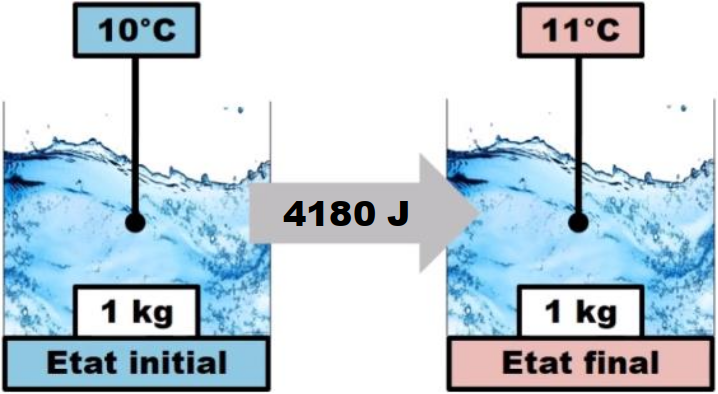
\includegraphics[scale = .2]{Ressources/TSPE_C14_Cours_Fig3b.png}&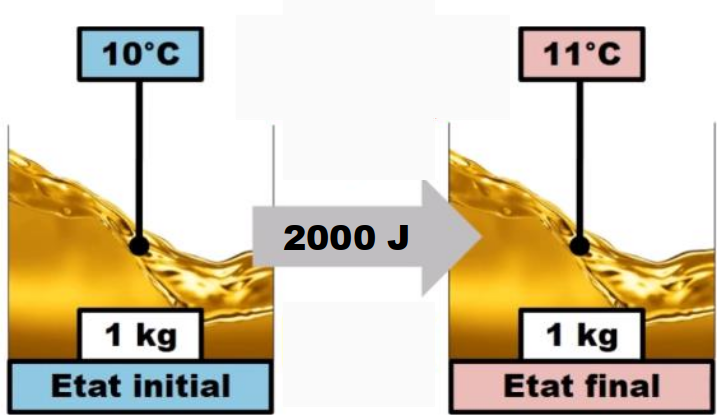
\includegraphics[scale = .2]{Ressources/TSPE_C14_Cours_Fig4b.png}\\
			\hline
	\end{tabular}
	\end{center}}
	
	\section{Transferts thermiques}
	\subsection{Modes de transfert}
	Trois modes de transfert thermiques peuvent avoir lieu, séparément ou simultanément :\\
	\begin{tabular}{|>{\centering}m{5cm}|>{\centering}m{5cm}|>{\centering\arraybackslash}m{8cm}|}
		\hline
		\textbf{Conduction thermique}&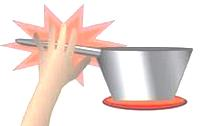
\includegraphics[scale = .35]{Ressources/TSPE_C14_Cours_Fig5.png}&Transfert de proche en proche, par des mouvements microscopiques des entités, mais sans déplacement macroscopique de matière. $\rightarrow$ \emph{dans les solides}\\
		\hline
		\textbf{Convection thermique}&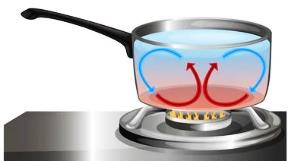
\includegraphics[scale = .25]{Ressources/TSPE_C14_Cours_Fig6.png}& Transfert généré par un mouvement d'ensemble d'un fluide. $\rightarrow$ \emph{dans les fluides (gaz ou liquides)}\\
		\hline
		\textbf{Rayonnement thermique}&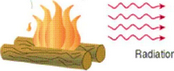
\includegraphics[scale = .35]{Ressources/TSPE_C14_Cours_Fig7.png}&transfert par absorption ou émission d'ondes électromagnétiques. $\rightarrow$ \emph{dans tous les milieux, y compris dans le vide}\\
		\hline
	\end{tabular}
	\subsection{Transfert thermique par conduction}
	la vitesse de transfert thermique (autrement dit le flux thermique) entre deux systèmes dépend de la \textbf{résistance thermique} de la paroi séparant les deux systèmes. Plus la résistance thermique de la paroi est élevée, plus le transfert thermique est lent (autrement dit plus le flux thermique est faible). La paroi sera alors plus isolante. Cela est traduit par la relation :\\
	
	\begin{tabular}{c|l}
		\multirow{3}{6cm}{\begin{equation*}
				\phi = \dfrac{T_A - T_B}{R_{th}} \text{ ou } R_{th} = \dfrac{T_A - T_B}{\phi}
		\end{equation*}}& $\phi$ : flux thermique (en W)\\
		&$R_{th}$ : résistance thermique (en \unit{\kelvin\per\watt\squared})\\
		&$T_A$ et $T_B$ : températures des deux systèmes (en \unit{\kelvin} ou en \unit{\celsius})\\
	\end{tabular}\\
	
	\noindent \begin{minipage}{.4\linewidth}
		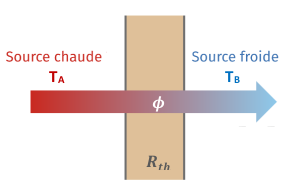
\includegraphics[scale=.6]{Ressources/TSPE_C14_Cours_Fig9.png}
	\end{minipage}
	\begin{minipage}{.5\linewidth}
		La résistance thermique d'une paroi dépend de sa constitution, de sa surface et de son épaisseur.
	\end{minipage}
	
	\subsection{Transfert thermique conducto-convectif}
	\noindent \begin{minipage}{.4\linewidth}
		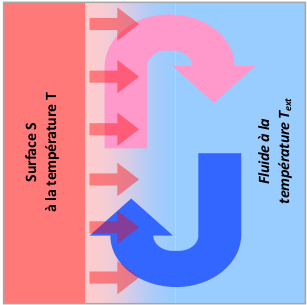
\includegraphics[scale=.6]{Ressources/TSPE_C14_Cours_Fig10.png}
	\end{minipage}
	\begin{minipage}{.6\linewidth}
		Un système en contact avec un fluide de température constante ( on par de \textbf{thermostat} échange de l'énergie avec ce fluide par conduction et par convection.\\
		A partir de ses observations expérimentales, Newton a établit que le flux thermique $\phi$ alors transféré à travers la surface $S$ du système vaut :\\
		\begin{tabular}{c|m{5cm}}
			\multirow{4}{5cm}{\begin{equation*}
					\phi = h \times S \times (T_{ext} - T)
			\end{equation*}}& $h$ : coefficient de transfert thermique (en \unit{\watt\per\meter\squared\per\kelvin}\\
			&$S$ : surface d'échange (en \unit{\meter\squared}\\
			&$T$ : température du système\\
			&$T_{ext}$ : température de l'extérieur (dans la même unité que $T$)\\
		\end{tabular}\\
		
		Cette loi est appelée \textbf{loi phénoménologique de Newton}.\\
	\end{minipage}
	
	Conséquence : lorsque l'écart de température entre un objet et l'extérieur est important, l'objet refroidit rapidement (flux thermique important). A mesure que cet écart diminue, le flux thermique baisse, l'objet refroidit donc de plus en plus lentement.\\
	
		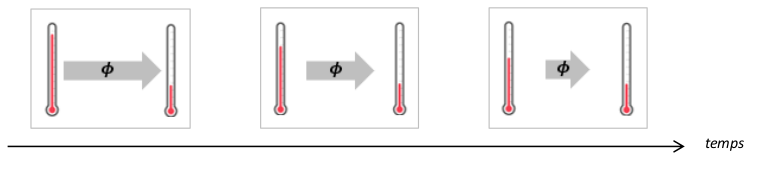
\includegraphics[scale=.6]{Ressources/TSPE_C14_Cours_Fig11.png}\\
	
	La température du système suit une décroissance exponentielle. Il est possible de le démontrer en établissant l'équation différentielle que vérifie cette température.

	\tabletail{\hline}
	\begin{xtabular}{|p{8cm}|p{10cm}|}
		\hline
		\multicolumn{2}{|c|}{\textbf{Bilan d'énergie}}\\
		\hline
		Définir le système.
		Schématiser les transferts d'énergie et indiquer leur signe. & \begin{center}
			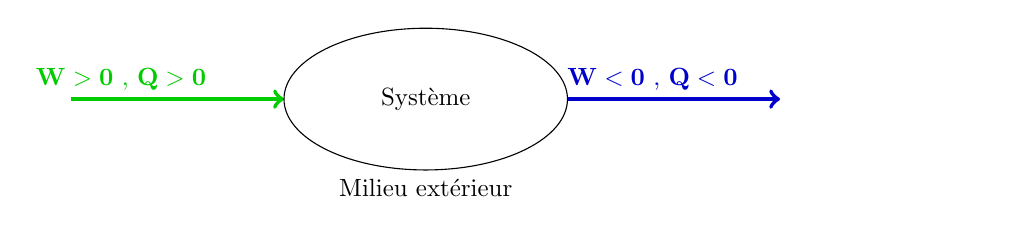
\begin{tikzpicture}[scale=.9,transform shape]
				\draw[green!80!black,->,line width=1.5] (-5,0) to (-2,0);
				\draw[blue!80!black,->,line width=1.5] (2,0) to (5,0);
				\draw (0,0) ellipse (2 and 1);
				
				\draw[green!80!black] (-2.5,0) node[above,text width=6cm]{$\mathbf{W>0}$ , $\mathbf{Q>0}$};
				
				\draw[blue!80!black] (5,0) node[above,text width=6cm]{$\mathbf{W<0}$ , $\mathbf{Q<0}$};
				
				\draw (0,0) node{Système};
				\draw (0,-1) node[below] {Milieu extérieur};
			\end{tikzpicture}\\
		\end{center} \\
		\hline
		\multicolumn{2}{|c|}{\textbf{Établissement de l'équation différentielle vérifiée par la température T}}\\
		\hline
		Exprimer le transfert thermique $Q$ à partir du premier principe de la thermodynamique. & D'après le premier principe de la thermodynamique :
		\begin{eqnarray}
			\Delta U = W + Q \nonumber\\
			\Delta U = Q \text{ car système immobile} \nonumber
		\end{eqnarray}\\
		Utiliser la variation d'énergie interne d'un système incompressible. & Or, pour un système incompressible,
		\begin{eqnarray}
			\Delta U = m \times c \times \Delta T \nonumber\\
			\text{Donc : } Q = m \times c \times \Delta T 
		\end{eqnarray}\\
		Exprimer le transfert thermique $Q$ en fonction du flux thermique & Par ailleurs, d'après l'expression du flux thermique : 
		\begin{eqnarray}
			Q = \phi \times \Delta t \nonumber
		\end{eqnarray}\\
		Remplacer le flux grâce à la loi phénoménologique de Newton. &
		Or, d'après la loi phénoménologique de Newton : 
		\begin{eqnarray}
			\phi = h \times S \times (T_{ext} - T) \nonumber
		\end{eqnarray}
		Donc : 
		\begin{eqnarray}
			Q = h \times S \times (T_{ext} - T) \times \Delta t 
		\end{eqnarray}
		On en déduit, en égalisant (1) et (2) que :
		\begin{eqnarray}
			m\times c \times \Delta T = h \times S \times (T_{ext} - T) \times \Delta t \nonumber
		\end{eqnarray}
		Pour un temps infiniment faible, il vient :
		\begin{eqnarray}
			m\times c \times dT = h \times S \times (T_{ext} - T) \times dt \nonumber\\
			m\times c \times \dfrac{dT}{dt} = h \times S \times (T_{ext}-T) \nonumber
		\end{eqnarray}
		On obtient une équation différentielle en T, que l'on peut écrire sous la forme $y'+ay=b$ :
		\begin{eqnarray}
			\dfrac{dT}{dt} + \dfrac{h\times S}{m \times c}\times T = \dfrac{h\times S}{m \times c} \times T_{ext} \nonumber
		\end{eqnarray}
		ou encore :
		\begin{eqnarray}
			\dfrac{dT}{dt} + \dfrac{1}{\tau}\times T = \dfrac{T_{ext}}{\tau} \text{ avec : } \tau = \dfrac{m\times c}{h\times S}\nonumber
		\end{eqnarray}\\
		\hline
		\multicolumn{2}{|c|}{\textbf{Résolution de l'équation différentielle}}\\
		\hline
		Trouver l'expression générale des solutions à cette équation. & Les solution de l'équation précédente sont de la forme :
		\begin{eqnarray}
			T(t)=K\times e^{-\dfrac{t}{\tau}} + T_{ext} \nonumber
		\end{eqnarray}\\
		Déterminer la solution particulière à l'aide des conditions initiales.& On détermine $K$ à l'aide des conditions initiales : à $t=0$, la température vaut $T_0$
		\begin{eqnarray}
			T(0)=T_0\nonumber\\
			K\times e^{-\dfrac{0}{\tau}}+T_{est}=T_0\nonumber\\
			K\times 1+T_{ext}=T_0\nonumber\\
			K=T_0-T_{ext}\nonumber
		\end{eqnarray}
		Ainsi :
		\begin{eqnarray}
			T(t)=(T_0-T_{ext})\times e^{-\dfrac{t}{\tau}} + T_{ext} \nonumber\\
			\text{avec le temps caractéristique } \tau = \dfrac{m\times c}{h\times S}\nonumber
		\end{eqnarray}\\
		\hline
		\multicolumn{2}{|c|}{\textbf{Allure de la courbe}}\\
		\hline
		\multicolumn{2}{|c|}{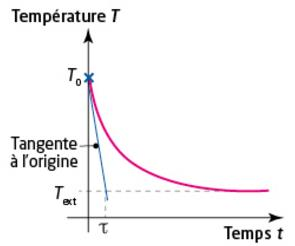
\includegraphics[scale=.8]{Ressources/TSPE_C14_Cours_Fig8.png}}\\
		\hline
	\end{xtabular}
\section{Bilan radiatif de la Terre}
	\subsection{Loi de Stefan-Boltzmann}
	Tour corps à température $T$ émet un rayonnement électromagnétique. La loi de Stefan-Boltzmann permet s'établir une relation entre le flux thermique surfacique émis $\varphi$ et la température $T$ :
	\begin{center}
		\begin{tabular}{c|l}
			$\varphi = \sigma \cdot T^4$ & $\varphi $ : flux thermique surfacique émis par un corps (\unit{\watt\per\meter\squared})\\
			& $\sigma$ : constante de Stefan-Boltzmann égal à $\sigma = \SI{5,67E-8}{\watt\per\meter\squared\per\kelvin\tothe{4}}$\\
			& $T$ : température du corps (\unit{\kelvin})\\		 
		\end{tabular}
		
	\end{center}
	
	\subsection{Bilan radiatif terrestre}
	Le rayonnement solaire parvenant jusqu'à la Terre est sa source principale d'énergie thermique. Comme la température moyenne de la surface de la Terre est stable au fil des ans, cela signifie que la surface reçoit en moyenne autant d'énergie qu'elle en émet vers l'espace par son propre rayonnement.\\
	La Terre reçoit un rayonnement solaire dont le flux thermique surfacique moyen est se l'ordre de $\varphi_S = \SI{340}{\watt\per\meter\squared}$. Environ $\alpha = \SI{30}{\percent}$ de ce rayonnement est réfléchi sans être absorbé par l'atmosphère : cette proportion est appelée \textbf{albédo}.\\
	Plus l'albédo est élevé, plus le rayonnement soplaire est réfléchi et moins la surface de la Terre reçoit d'énergie thermique.\\
	Si une partie du rayonnement émis par la Terre n'était pas absorbée par l'atmosphère, la température à sa surface serait d'environ \SI{-18}{\celsius}. Cette absorption est principalement sue à la présence s'eau et de dioxyde de ccarbone dans l'atmosphère créant ce que l'on nomme \textbf{l'effet de serre}.
	\begin{center}
		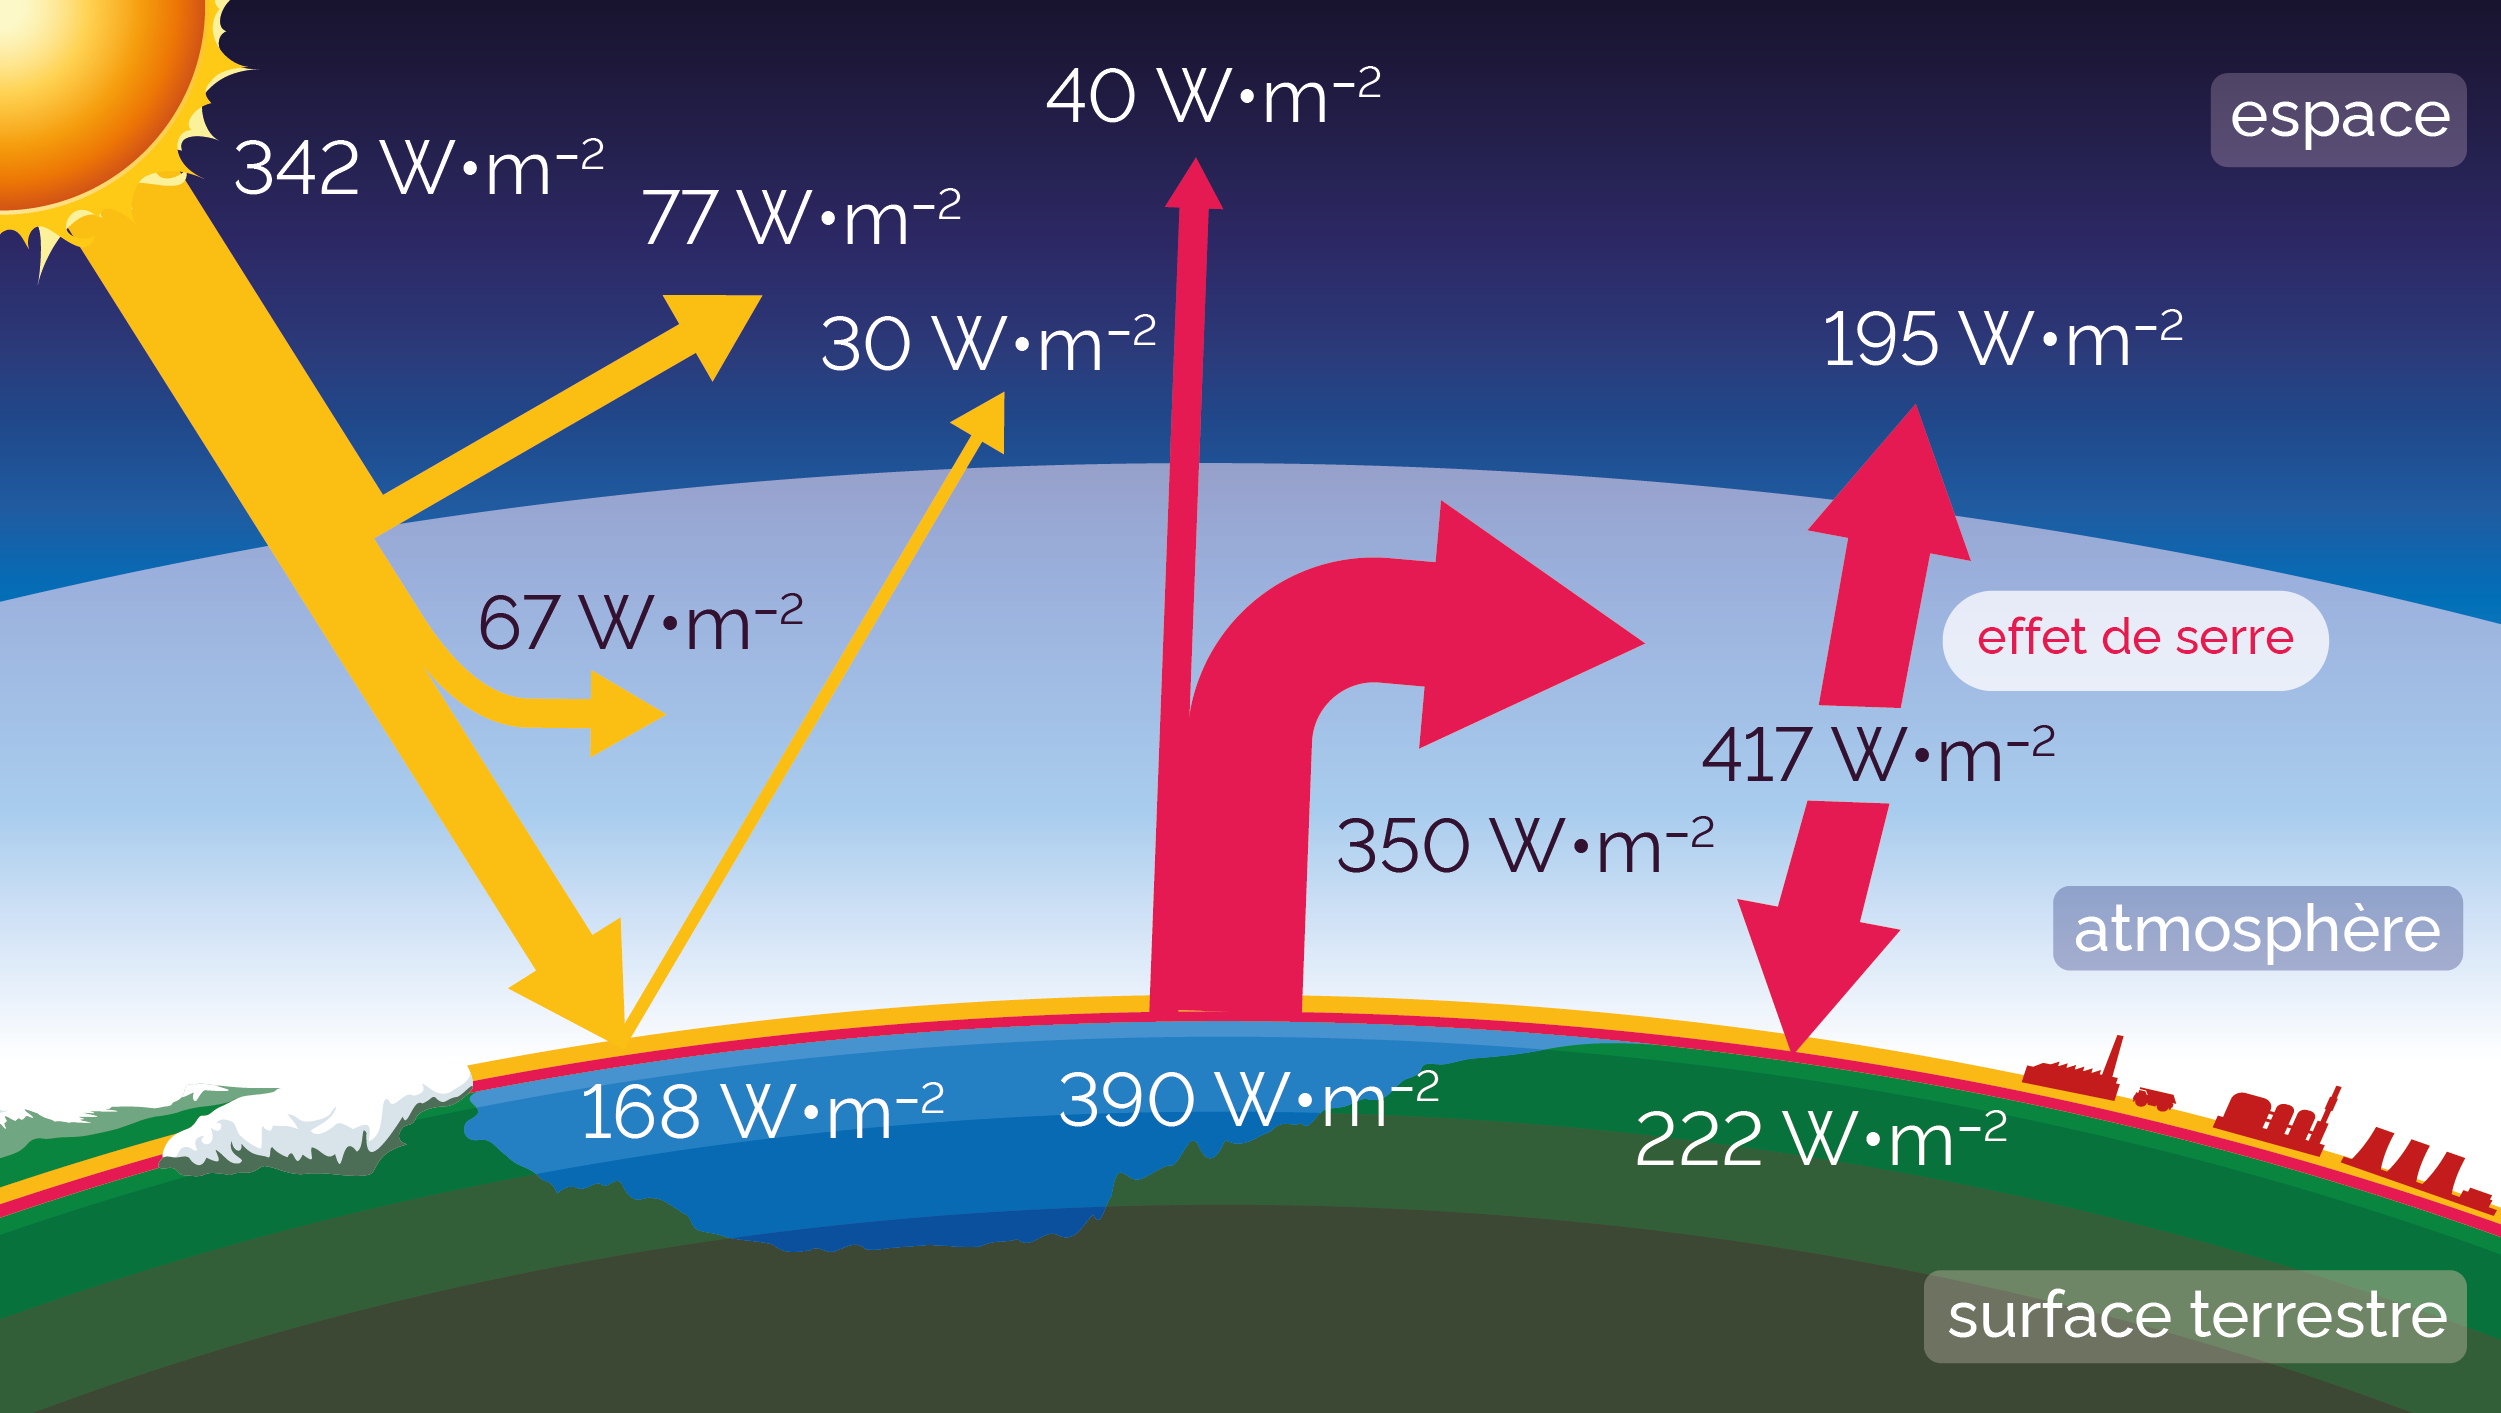
\includegraphics[width=.7\linewidth]{Ressources/proxy-image.png}
	\end{center}
	

\end{document}